\section{Dienstag}

\subsection{Lehrinhalte FOPT3 und FOPT4}

\subsubsection{Notizen zu den Lehrinhalten FOPT3 und FOPT4}

\subsubsection*{UML}
\begin{itemize}
    \item Klassendiagramme
    \begin{itemize}
        \item Assoziationen mit und ohne Kardinalitäten
        \item Benutzt-Beziehungen
        \item Implementierungsbeziehungen
        \item Vererbungsbeziehungen
    \end{itemize}
    \item Objektdiagramme
    \item Sequenzdiagramme
\end{itemize}

\subsubsection*{Einführung in die Programmierung mit JavaFX}

\paragraph*{Allgemein}

\begin{itemize}
    \item Inhalt eines Fensters
    \begin{itemize}
        \item Baumartige Struktur aus Containern (Layout)
        \item Sichtbare Interaktionselemente (Labels, Buttons, Texteingabefelder, Slider usw.)
    \end{itemize}
    \item Anwendung kann mehrere Fenster erzeugen
\end{itemize}

\paragraph*{"Kochrezept" für JavaFX-Programm}

\begin{itemize}
    \item Ableiten aus Klasse Application
    \item Überschreiben der Methode start mit Parameter Stage
    \begin{itemize}
        \item Initialisierung der Oberfläche
        \item Aufbau der Baumstruktur
        \item Anmeldung von Ereignisbehandlern
        \item Übergabe der Wurzel des Baums an eine Scene
        \item Einfügen der Scene in die Stage
        \item Angabe eines Titels für das Fenster
        \item Anzeigen des Fensters (show)
    \end{itemize}
    \item Main-Methode mit Aufruf von launch
    \item Kommandozeilenargumente
    \item FXML
\end{itemize}

\paragraph*{Grundlagen: Properties, Bindings und JavaFX-Collections}

\begin{itemize}
    \item Property-Konzepte
    \begin{itemize}
        \item Kapselung eines Werts
        \item Anmeldung von Beobachtern bei Wertänderung
        \item ReadOnlyProperty und ReadOnlyWrapper
        \item[](ReadOnlyWrapper wird genutzt, wenn eine Property von Außen nicht geändert werden darf, es aber trotzdem möglich sein soll, einen Listener an der Property zu registrieren.)
    \end{itemize}
    \item Bindings
    \begin{itemize}
        \item Kopplung von Properties
        \item Unidirektional oder bidirektional
        \item Kopplungsnetze über Operationen
    \end{itemize}
    \item JavaFX-Collections
    \begin{itemize}
        \item Listen und HashMaps
        \item Wie Properties beobachtbar
    \end{itemize}
\end{itemize}

\paragraph*{Elemente von JavaFX}

\begin{itemize}
    \item Container und Interaktionselemente
    \begin{itemize}
        \item Verschiedene Arten von Panes und Layouts
        \item[](Pane, VBox, HBox,...; i.d.R. sind das die ``root``-Elemente)
        \item Label, Button, CheckBox, RadioButton, ComboBox, ListView, Slider, TextField, PasswordField, TextArea, TableView, TreeView, TreeTableView
    \end{itemize}
    \item Grafikprogrammierung
    \begin{itemize}
        \item Paint, Color, LinearGradient, RadialGradient, ImagePattern
        \item Shape, Line, Rectangle, Circle, Ellipse, Polyline, Polygon, Arc, QuadCurve, CubicCurve, Text
        \item Pane als empfohlener Container für Shape-Objekte
        \item Interaktion und Clipping
        \item[] (Clipping-Maske kann relativ einfach über ein \code{Rectangle} und der Methode \code{setClip(c: Rectangle)} realisiert werden, s.a.\cite[222]{Oec22})
    \end{itemize}
\end{itemize}

\paragraph*{Architekturmuster MVP}

\begin{itemize}
    \item Unterscheidung Architekturmuster und Entwurfsmuster
    \item Komponenten: Modell, Darstellung, Präsentationssteuerung
    \item[] (Presenter = ``Ablaufsteuerungskomponente``)
    \item Isoliertes Testen der Komponenten
    \item Mehrere Views, Presenter und Modelle möglich
\end{itemize}

\paragraph*{Anwendungen mit mehreren Fenstern}

\begin{itemize}
\item Erzeugung und Anzeige neuer Stage-Objekte
\item Stage-Properties: x, y, width, height, resizable
\item Init-Methoden von Stage: StageStyle, Owner, Modality
\item Methoden außer show: showAndWait
\end{itemize}

\paragraph*{Dialoge}

\begin{itemize}
    \item Ähnlichkeit zu Stage, aber keine Vererbungsbeziehung
    \item Spezielle Dialogklassen: Alert, TextInputDialog, ChoiceDialog
\end{itemize}

\paragraph*{Undo-Redo}

\begin{itemize}
    \item UndoRedoManager basierend auf dem Entwurfsmuster Command
    \item Integration in die Presenter-Komponente
\end{itemize}

\paragraph*{Parallele Programmierung und grafische Benutzeroberflächen}

\begin{itemize}
    \item Regel 1: Ereignisbehandlung muss kurz sein
    \item Regel 2: Zugriff auf Oberflächenelemente nur durch den "JavaFX Application Thread"
    \item Delegation von Oberflächenzugriffen durch andere Threads mittels Platform.runLater
    \item Realisierung mit Basismechanismen oder Klassen Task, Service, ScheduledService
    \item[] (Der \textbf{JavaFX Application Thread} ist der Thread, dem Zugriff auf die Oberfläche gestattet ist. Führt man in diesem Thread Berechnungen durch, hat der Thread keine Gelegenheit, gleichzeitig die UI zu aktualisieren - deshalb sollten länger andauernde Berechnungen in einen eigenen Thread ausgelagert werden; das Ergebnis der Berechnung kann dann über \code{Platform.runLater()}, dem ein \code{Runnable} übergeben wird, in der UI dargestellt werden. Da nur der \code{JavaFX Application Thread} auf die UI zugreifen darf, \textit{muss} die Methode aus einem anderen Thread so aufgerufen werden.)
\end{itemize}

\paragraph*{Animationen}

\begin{itemize}
    \item Realisierung mit Basismechanismen oder Transitions und/oder Timelines
\end{itemize}




\subsection{Notizen}

\subsection*{UML}

\begin{figure}
    \centering
    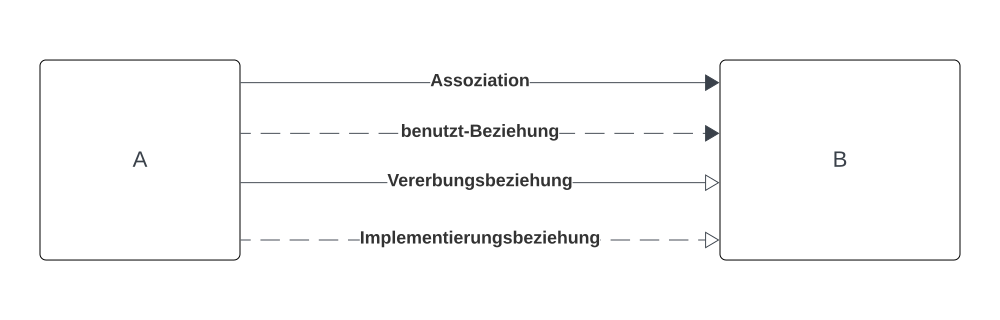
\includegraphics[scale=0.5]{chapters/Anhang/Präsenzphase/img/umldependencies}
    \caption{Abhängigkeitsbeziehungen und die im Kurs verwendete Notation.
    Die Pfeilrichtung drückt die Abhängigkeitsrichtung aus: $A$ ist in allen 4 Fällen abhängig von $B$. Ändert sich $B$, muss sich auch $A$ ändern. (Quelle: eigene)}
    \label{fig:umldependencies}
\end{figure}


\subsection*{ToggleGroups}
\code{RadioButton}s lassen sich über eine \code{ToggleGroup}\footnote{
``Class ToggleGroup``: \url{https://docs.oracle.com/javase/8/javafx/api/javafx/scene/control/ToggleGroup.html} - abgerufen 20.2.2024
} gruppieren:

\begin{minted}[mathescape,
    linenos,
    numbersep=5pt,
    gobble=2,
    frame=lines,
    framesep=2mm]{java}
    RadioButton one = new RadioButton("one");
    RadioButton two = new RadioButton("two");
    RadioButton three = new RadioButton("three");

    ToggleGroup radioButtonGroup = new ToggleGroup();
    radioButtonGroup.getToggles().addAll(one, two, three);
\end{minted}\\

\subsection*{StringProperty an IntegerProperty binden}

\begin{center}\code{Bindings.convert(observableValue: ObservableValue<?>): StringExpression}\end{center}
ermöglicht es, bsp. ein JavaFX-\code{Label} an eine \code{SimpleIntegerProperty} zu binden\footnote{
``convert``: \url{https://docs.oracle.com/javase/8/javafx/api/javafx/beans/binding/Bindings.html#convert-javafx.beans.value.ObservableValue-} - abgerufen 20.2.2024
}.\\

\noindent
Das Folgende Beispiel bindet 3 Labels an drei verschiedene \code{SimpleIntegerProperty}s.\\
Die Summe dieser Properties wird in dem Label \code{totalLabel} angezeigt:
\begin{minted}[mathescape,
    linenos,
    numbersep=5pt,
    gobble=2,
    frame=lines,
    framesep=2mm]{java}
    Label lineCountLabel = new Label();
    Label rectangleCountLabel = new Label();
    Label circleCountLabel = new Label();
    Label totalLabel = new Label();

    lineCountLabel.textProperty().bind(Bindings.convert(lineCountProperty));
    rectangleCountLabel.textProperty().bind(Bindings.convert(
        rectangleCountProperty
    ));
    circleCountLabel.textProperty().bind(Bindings.convert(circleCountProperty));

    totalLabel.textProperty().bind(
        Bindings.convert(
            lineCountProperty.add(rectangleCountProperty).add(
                circleCountProperty
            ))
    );
\end{minted}\\

\subsection*{Stage Owner}

Mit \code{initOwner(owner: Window)}\footnote{
``initOwner``: \url{https://docs.oracle.com/javase/8/javafx/api/javafx/stage/Stage.html#initOwner-javafx.stage.Window-} - abgerufen 20.2.2024
} läßt sich der \textbf{Owner} eines Windows festlegen.
Das Fenster, auf das \code{initOwner()} aufgerufen wurde, wird dann bspw. geschlossen, wenn der Owner geschlossen wird:

\blockquote[{\url{https://docs.oracle.com/javase/8/javafx/api/javafx/stage/Stage.html} - abgerufen 20.2.2024}]{
    A stage can optionally have an owner Window. When a window is a stage's owner, it is said to be the parent of that stage. When a parent window is closed, all its descendant windows are closed. The same chained behavior applied for a parent window that is iconified. A stage will always be on top of its parent window. The owner must be initialized before the stage is made visible.
}

\subsection*{ObservableList: removeAll() vs. clear()}

Als Alternative zu der Methode \code{removeAll(c: Collection<?>)} des Interface \code{java.util.List<E>}\footnote{
``Interface List<E>``: \url{https://docs.oracle.com/en/java/javase/21/docs/api/java.base/java/util/List.html} - abgerufen 20.2.2024
} bietet die davon abgeleitete Schnittstelle \code{ObservableList<E>} aus dem Package \code{javafx.collections} die Methode
\code{removeAll(elements:E...)}\footnote{
    ``removeAll``\url{https://docs.oracle.com/javase/8/javafx/api/javafx/collections/ObservableList.html#removeAll-E...-} - abgerufen 20.2.2024
} an, die einen Aufruf mit \textbf{variabler Argumentanzahl}\footnote{
    ``8.4.1. Formal Parameters - VariableArityParameter``:  \url{https://docs.oracle.com/javase/specs/jls/se21/html/jls-8.html#jls-VariableArityParameter} - abgerufen 20.2.2024
} erlaubt.\\

\noindent
Hierbei ist zu beachten, dass ein Aufruf von \code{removeAll()} ohne Argumente \textit{nicht} automatisch alle Objekte aus der Liste löscht, wie man aufgrund der semantischen Bedeutung der Methode vermuten könnte.\\
Hierzu sollte stattdessen die Methode \code{clear()}\footnote{
``clear``: \url{https://docs.oracle.com/en/java/javase/21/docs/api/java.base/java/util/List.html#clear()} - abgerufen 20.2.2024
} verwendet werden.


\subsection*{Undo-Redo}

Undo-Redo orientiert sich an dem \textbf{Command}-Pattern\footnote{
    ``Command Pattern``: \url{https://en.wikipedia.org/wiki/Command_pattern} - abgerufen 24.02.2024
}.\\
Der \textit{UndoRedo}-Manager speichert in seiner Liste Objekte, die die Schnittstelle \textit{Action} implementieren.\\
Jede \textit{Action} verfügt über die Methode \code{undo()} / \code{redo()}, deren Implementierungsdetails unbekannt sind.\\
Die logische Position der Liste ist i.d.R. ``zwischen`` zwei Actions, die konkrete Position die jeweils aktuelle Action.\\
Wird ein \code{redo()} aufgerufen, und befindet sich rechts der logischen Listenposition ein Element, wird auf diesem Element die Aktion \code{redo()} ausgeführt.
Der Listenzeiger wandert dann um eins nach rechts.\\
Wird \code{undo()} aufgerufen, und es befindet sich links der logischen Position ein Element, wird auf diesem Element \code{undo()} aufgerufen, und der Listenzeiger wandert um eins nach links, falls möglich (s. Abbildung \ref{fig:undoredo}).

\begin{minted}[mathescape,
    linenos,
    numbersep=5pt,
    gobble=2,
    frame=lines,
    framesep=2mm]{java}
    class UndoRedoManager {
        public function add(Action a) {
            for (int i = actions.size() - 1; i >= currentPos; i--) {
                actions.remove(i);
            }
            actions.add(a);
            currentPos++;
        }
        public function undo() {
            if (currentPos == 0) {
                return;
            }
            currentPos--;
            actions.get(currentPos).undo();
        }
        public function redo() {
            if (currentPos == actions.size()) {
                return;
            }
            actions.get(currentPos).redo();
            currentPos++;
        }
    }
\end{minted}\\

\begin{figure}
    \centering
    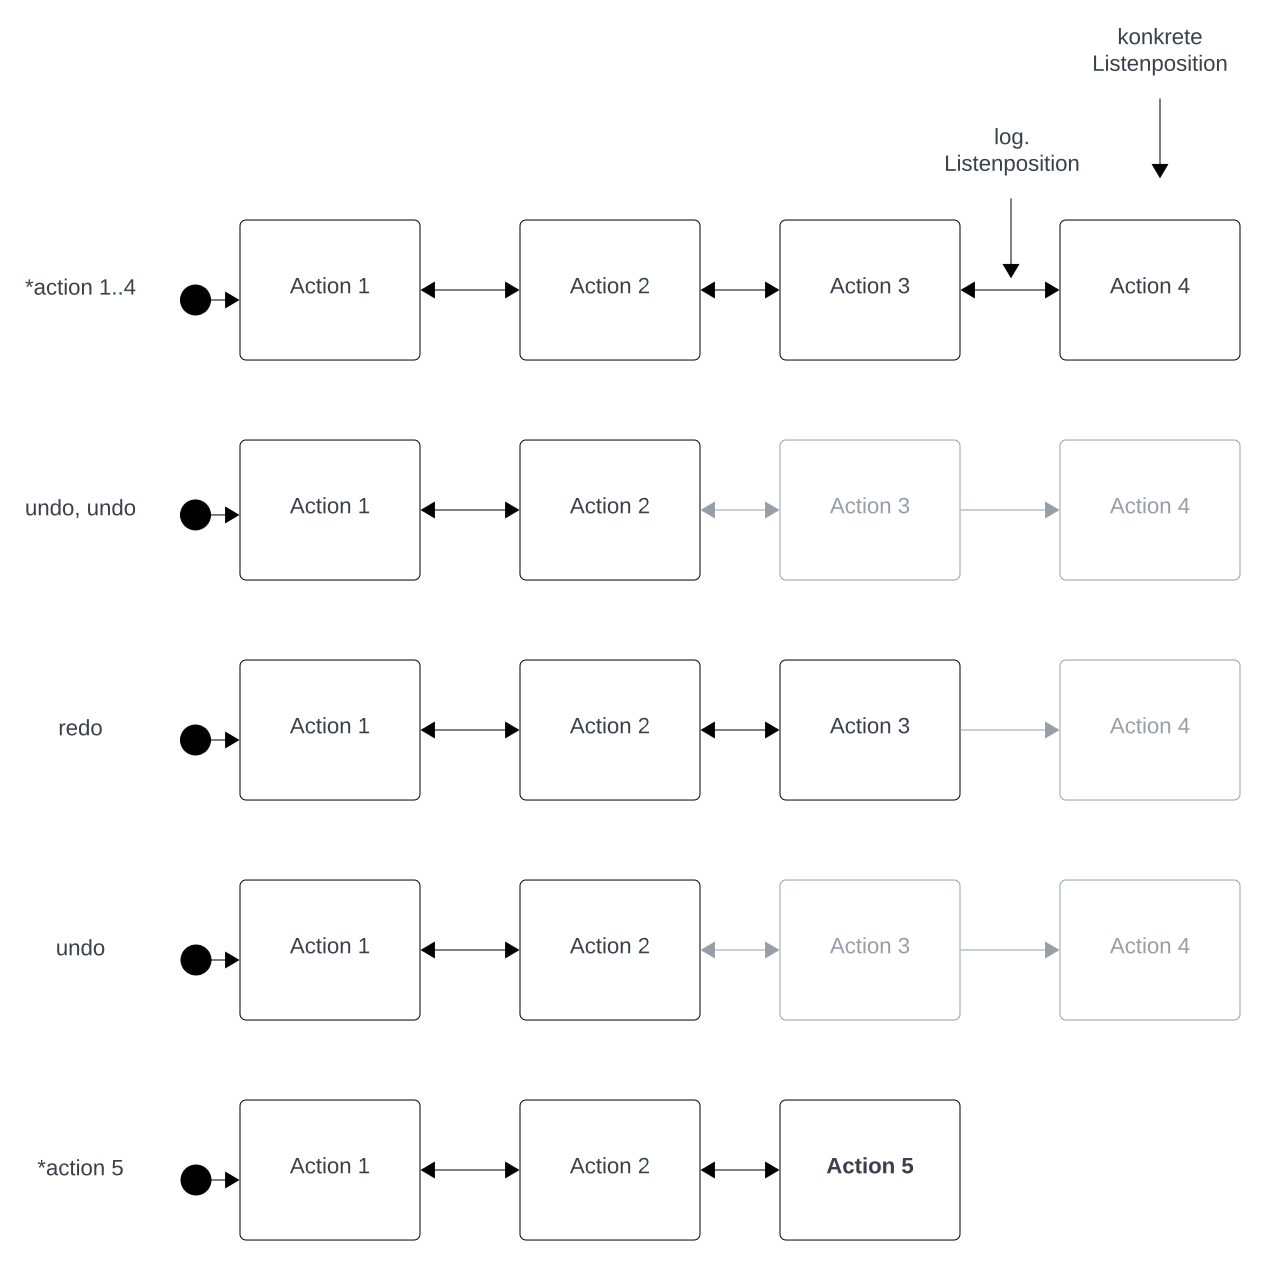
\includegraphics[scale=0.25]{chapters/Anhang/Präsenzphase/img/undoredo}
    \caption{Schematische Darstellung von undo/redo Operationen. Sobald man sich in der Historie rückwärts bewegt, und eine neue Aktion ausgeführt wird, werden nachfolgende Einträge gelöscht. (Quelle: eigene)}
    \label{fig:undoredo}
\end{figure}